%\titleformat{\chapter}[display]
 % {\normalfont\huge\bfseries}{\chaptertitlename\ \thechapter}{1em}%{\Huge}
 \newpage
 \pagenumbering{arabic}

\patchcmd{\chapter}{\thispagestyle{plain}}{\thispagestyle{fancy}}{}{}
 \fancypagestyle{main}{
  \fancyhf{} % clear all header and footer fields
  \renewcommand{\headrulewidth}{0pt} % remove header rule
  \renewcommand{\footrulewidth}{1pt} % set footerr rule
  \fancyfoot[L]{\fontsize{11}{13}\selectfont \leftmark} % chapter name at left footer
  \fancyfoot[R]{Page \thepage\ of \pageref{LastPage}} % page number at center footer
}
\pagestyle{main} % set the main page style
\setcounter{page}{1}

%  \titleformat{\chapter}{\Huge}{\chaptertitlename \ \thechapter :}
%  {1em}{}[\vspace{-1.1em}\underline{\hspace{\linewidth}}]

% % Define style for section headings
% \titleformat{\section}[block]
%   {\normalfont\Large\bfseries}{\thesection}{1em}{}

% % Define style for subsection headings
% \titleformat{\subsection}
%   {\normalfont\large\bfseries}{\thesubsection}{1em}{}

% Define style for equation numbers
\renewcommand{\theequation}{\arabic{chapter}.\arabic{equation}}

\chapter{INTRODUCTION}
\section{Background}
The increasing demand for faster data transfer rates and dependable connectivity in numerous applications, including 5G networks, satellite communications, and radar systems, has been driving the demand for high-performance wireless communication systems. Power amplifiers are essential in these systems for supplying enough power and amplification to permit effective signal transmission. The intrinsic constraints of the complementary metal-oxide-semiconductor (CMOS) technology, however, make it difficult to create power amplifiers that can function well in the millimeter-wave frequency range.

Since the debut of the first contemporary mobile phone system, the wireless communication market has grown and developed in an impressive manner, with a steady rise in subscribers, new application areas, and higher data rates. A number of enormous improvements in
semiconductor technology have been made as a result of the expansion of the wireless communication sector. The most notable development among them is in CMOS technology. Transistors have the surprising advanced property of increasing speed while using less power
per function in digital circuits and costing less as their size is lowered. These CMOS technology breakthroughs have therefore significantly improved the performance and functionality of contemporary mobile devices.
\begin{figure}[h]
    \centering
    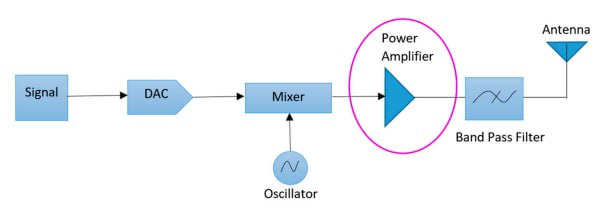
\includegraphics{figures/rf-transmitter-block-diagram.jpeg}
    \caption{Basic block diagram of radio frequency (RF) transmitter \cite{first}.}
    \label{fig:rf-transmitter-block-diagram}
\end{figure}

The development of complementary metal-oxide semiconductor (CMOS) technology, which has greater advantages than gallium arsenide (GaAs) and gallium nitride (GaN) technologies, has led to a rapid increase in the use of wireless communication systems \cite{second,third}. As a result of the compact chip size and ability to operate at a lower power supply, CMOS technology minimizes fabrication costs \cite{fourth} and circuit power dissipation. Radio frequency (RF), digital,
and analog functionalities may be inexpensively combined on a single chip using CMOS \cite{fifth}.
\begin{figure}[h]
    \centering
    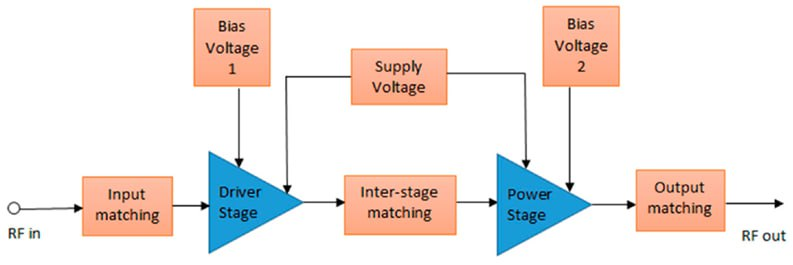
\includegraphics[]{figures/cmos-power-amplifier-block-diagram.jpeg}
    \caption{Block diagram of complementary metal–oxide semiconductor (CMOS) power
amplifier \cite{sixth}.}
    \label{fig:cmos-power-block-diagram}
\end{figure}

For contemporary wireless devices, the CMOS power amplifier (PA) is a potential option to meet the demand for a low-power and low-cost design. In numerous wireless communication applications throughout the years, including home automation, Radio Frequency Identification (RFID), industrial consumer electronics, TV transmissions, phones, and
medical equipment \cite{fourth, fifth, seventh}. CMOS PA has been widely used due to the need for a higher contrast resolution in ultrasonic imaging, which can be achieved by a highly linear PA , it has been integrated in high-frequency medical ultrasonic applications to amplify high-voltage excitation signals to activate ultrasonic transducers \cite{sixth}.

One approach to achieving high efficiency in a wide band power amplifier is to use a two stage amplifier design. In this design, the first stage amplifies the input signal and the second
stage provides additional gain and power. By using a two-stage design, the amplifier can
achieve high efficiency while maintaining good linearity and low distortion \cite{ninth}.

Another approach to achieving high efficiency in a power amplifier is to use a superimposed dual-band configuration. This configuration involves combining two different frequency bands into a single amplifier, which can improve efficiency by reducing the number of
amplifiers required \cite{tenth}.

The use of 90 nm CMOS technology in the design of the power amplifier allows for high levels of integration and miniaturization, making it suitable for use in small devices such as mobile phones and wireless sensors. The use of this technology also enables high levels of
performance in terms of power efficiency and linearity \cite{eleventh}.

\section{Thesis Objectives}
The main objectives of the works are:
\begin{enumerate}[label=\roman*. ]
  \item To increase gain of power amplifier using two stage CMOS power amplifier.
  \item To maintain wideband performance of the amplifier.
  \item To design input and interstage matching network for impedance matching.
\end{enumerate}
 
\section{Context}
The thesis paper titled "Design and of CMOS Power Amplifiers for Enhanced Gain and Bandwidth Using 90 nm CMOS Technology" focuses on the design, simulation, and implementation of a power amplifier that operates in the frequency range of \SI{25}{\giga\hertz} - \SI{35}{\giga\hertz}.

The \SI{25}{\giga\hertz} - \SI{35}{\giga\hertz} frequency range has gained significant attention in various sectors,
including telecommunications, radar systems, and satellite communications. The high frequency range allows for high-speed data transfer and communication, making it suitable
for 5G networks, Internet of Things (IoT), and other wireless applications. Furthermore, the
use of this frequency range is critical in advanced radar systems, such as automotive and
aerospace radar, for precise detection and tracking of objects.

Despite the importance of this frequency range, the design of a power amplifier that meets the
requirements of high power, high efficiency, and wide bandwidth is challenging. The primary
difficulty is the trade-off between power, efficiency, and bandwidth. Increasing the power
amplification often results in lower efficiency, while expanding the bandwidth typically leads
to decreased power output. Moreover, designing a power amplifier that operates in a
superimposed dual-band configuration adds further complexity to the system.

Thus, the statement of the problem situation for this thesis is the difficulty of designing a
power amplifier that meets the requirements of high power, high efficiency, and wide
bandwidth in a superimposed dual-band configuration using 90 nm CMOS technology. The
areas of concern include the selection of an appropriate transistor model, the design of
matching networks, and the optimization of biasing conditions to achieve the desired
performance. The felt need for this research is to provide a solution that overcomes the
challenges of designing a power amplifier for the \SI{25}{\giga\hertz} - \SI{35}{\giga\hertz} frequency range, which is
crucial for many advanced wireless and radar applications.

\section{Significance \& Scope}
\subsection{Significance}
The demand for high-speed wireless communication systems has increased significantly in
recent years. The need for high-frequency wideband power amplifiers (PAs) has become
critical in meeting this demand. The proposed 2-stage high power gain and wideband
(\SI{25}{\giga\hertz} - \SI{35}{\giga\hertz}) power amplifier using superimposed dual-band configuration using 90 nm
CMOS technology aims to address this need. The study is significant in that it provides a
solution for high-frequency wireless communication systems with high gain and
wideband capability.

\subsection{Gap in the Literature}
Although there have been studies on wideband PAs, there is limited research on high frequency wideband PAs using superimposed dual-band configuration.Numerous benefits of CMOS technology include affordability, low power usage, and interoperability with methods used to manufacture integrated circuits. For the creation of power
amplifiers for millimeter-wave applications, it therefore has enormous promise. However,
CMOS power amplifiers struggle to achieve high gain and wide bandwidth due to a number
of challenges, including parasitic capacitances, frequency-dependent transconductance, and
impedance matching problems.

In order to overcome these obstacles and investigate approaches for building and enhancing CMOS power amplifiers, this study will focus on the millimeter-wave frequency range. The main goal is to create power amplifier topologies and strategies that can get around CMOS technology's constraints and provide better performance.

The study's foundational assumptions will be examined, along with the effects of parasitic capacitances and frequency-dependent transconductance on the gain and bandwidth characteristics of CMOS power amplifiers. This research will shed light on the underlying variables affecting the performance of the amplifier and serve as a roadmap for the ensuing design and optimization process.

A multi-stage technique will be used to increase gain and bandwidth, where extra amplifier stages will be cascaded to make up for the shortcomings of individual stages. The frequency response and linearity of the power amplifier will be enhanced by employing a staggered tuning method.

In order to overcome problems with impedance matching, matching networks will be created and implemented into the power amplifier architecture. These networks will make sure that the amplifier and the linked components transmit power effectively, increasing gain and lowering return loss as a result.


\subsection{Scope \& Delimitations}
Numerous benefits of CMOS technology include affordability, low power usage, and interoperability with methods used to manufacture integrated circuits. For the creation of power amplifiers for millimeter-wave applications, it therefore has enormous promise. However, CMOS power amplifiers struggle to achieve high gain and wide bandwidth due to a number of challenges, including parasitic capacitances, frequency-dependent transconductance, and impedance matching problems.

In order to overcome these obstacles and investigate approaches for building and enhancing CMOS power amplifiers, this study will focus on the millimeter-wave frequency range. The main goal is to create power amplifier topologies and methods that can get around CMOS technology's constraints and provide better performance.

\section{Classifications of PA}
\subsection{Class-A, AB, B, and C Power Amplifiers}
The fundamental difference between these four power amplifiers' circuit designs is how they are biased. The class-A power amplifier is demonstrated in Figure \ref{fig:general-topology-PA} to function as a small-signal amplifier, offering linear amplification for the whole input cycle without clipping. As a result, the output closely matches the enlarged input.

However, class-A amplifiers waste power in order to achieve this high level of linearity. The idea of "reduced conduction angle" was developed to increase efficiency while preserving sufficient linearity. In order to implement this idea, active devices are biased with low quiescent current and only partially activated by the input RF signal throughout each cycle.

The amplifier switches from class-AB to class-B and then to class-C by reducing the conduction angle. The active components function as current sources regardless of the conduction angle, giving them the name "transconductance" power amplifiers \cite{twelveth}.

\begin{figure}[h]
    \centering
    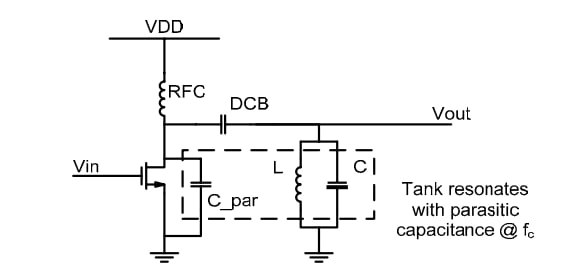
\includegraphics{figures/general-A-B-AB-C.jpeg}
    \caption{A generic topology for class-A, AB, B, and C power amplifiers \cite{twelveth}.}
    \label{fig:general-topology-PA}
\end{figure}

\subsection{Class-D Power Amplifiers}
A class D amplifier is an amplifier that employs a voltage-controlled switch and a filtering tank to amplify a signal. The output tuned network of the amplifier is engineered to exhibit minimal impedance at the fundamental frequency and high impedance at harmonic frequencies. This simplifies the analysis of the amplifier since the drain voltage waveform is straightforward. Under ideal operating conditions, the drain efficiency of the amplifier can reach 100\%, comparable to that of other types of switching power amplifiers \cite{twelveth}.

\begin{figure}[h]
    \centering
    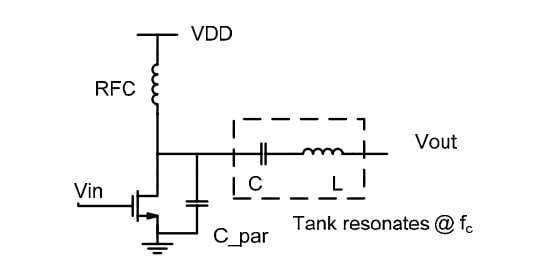
\includegraphics{figures/class-D.jpeg}
    \caption{A voltage switching class-D amplifier \cite{twelveth}.}
    \label{fig:class-D-amplifier}
\end{figure}

\subsection{Class-E Power Amplifier}
The Class-E power amplifier stands out among other switching power amplifiers due to its distinctive capability of incorporating the parasitic capacitances of active devices into wave-shaping and matching networks, resulting in high efficiency. In Figure \ref{fig:class-E-amplifier}, the simplest form of Class-E power amplifiers is depicted, operating by manipulating the drain current and voltage waveforms to prevent overlap. Moreover, the voltage gradually diminishes to zero prior to the activation of the active device, enhancing efficiency by avoiding the charging and discharging of capacitors at the drain. Nevertheless, one limitation of the Class-E power amplifier is its elevated peak voltage.
\begin{figure}[h]
    \centering
    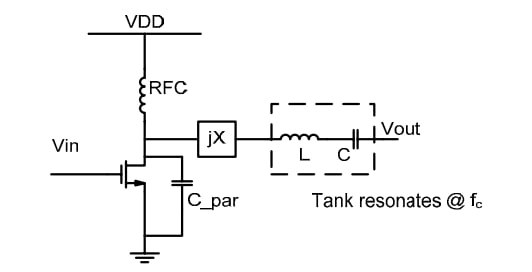
\includegraphics{figures/class-E.jpeg}
    \caption{A simple class-E amplifier \cite{twelveth}}
    \label{fig:class-E-amplifier}
\end{figure}

\subsection{Class-F Power Amplifier}
Class-F amplifiers are recognized for their utilization of a load network that generates resonance at various harmonic frequencies, including the fundamental frequency. Initially, these amplifiers were proposed to enhance the efficiency of overdriven transconductance amplifiers. The active devices employed in class-F amplifiers typically operate as transconductors or current sources.

However, under high input drive conditions, these devices can exhibit switch-like behavior akin to that observed in switching amplifiers. In practical scenarios, it is uncommon to encounter class-F amplifiers with tuned harmonics surpassing the 5th harmonic. This is primarily due to the intricacy associated with designing a waveform shaping network using lumped elements.

\begin{figure}[h]
    \centering
    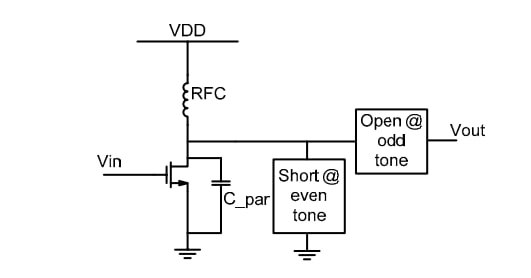
\includegraphics{figures/class-F.jpeg}
    \caption{A class-F power amplifier with tuned harmonics for waveform shaping \cite{twelveth}.}
    \label{fig:my_label}
\end{figure}
\section{Performance Parameter}
Multiple parameters were used to assess the CMOS PA's performance. The output power,
power consumption, power gain, linearity, and power added efficiency (PAE) of a PA design
are its most crucial components. These aspects inevitably come with trade-offs, and as a
result, PA design for CMOS downscaling is difficult. These were the main criteria that were
used for measuring performance.

\subsection{Output Power}
The output power (Pout) \cite{third} is the amount of power sent to the load, which is the antenna. Higher power output must be achieved at the expense of efficiency because some power is lost as heat. To account for this power loss, the device's energy supply must be greater than its needed output power \cite{fourtheen}. The current is essential for maintaining a consistent supply voltage and achieving the necessary output power. As a result, the output power of the power amplifier (PA), which is directly related to the PA's efficiency, determines the PA's performance. The output power is transformed into its appropriate dBm value using the following equation:

\begin{equation}
    P_{out}=\frac{V_{out}^2}{2R_L}
\end{equation}

Where $V_{out}$ denotes the output voltage and $R_L$ denotes the resistance load.
\subsection{Power Consumption}
The power consumption of a power amplifier (PA) is another important aspect of its performance. It's critical to address the need for extended battery life without sacrificing excessive power consumption given the rising demand for portable devices. According to the first equation, the PA's total power consumption ($P_{Total}$) is calculated by adding its dynamic and static power consumption. Leakage current ($I_{CC}$) causes static power consumption $(P_S)$, whereas high-frequency switching causes dynamic power consumption ($P_D$). The two equations that follow show how to determine static and dynamic power usage. Reduced heat generation inside the device is a direct result of reduced static power, which has a major impact on overall power usage. In addition to reducing the device's exposure to heat, this decrease in power consumption increases system dependability. To extend battery life, PAs must use as little electricity as possible because excessive power utilization can reduce their longevity.
\begin{align}
    P_{Total}&=P_S+P_D\\
    P_S&=V_{DD}\times I_{CC}
\end{align}

\begin{equation}
    P_D=\left[\left(C_{pd}\times f_I\times N_{SW}\right)+ \sum \left(C_{Ln}\times f_{On}\right) \right]
\end{equation}

The power consumption capacitance is denoted in the context by $C_{pd}$ (in Farads). In Hertz, $f_I$ stands for the input frequency, while $f_{On}$, also in Hertz, is the total frequency of all outputs at each output. $N_{SW}$ stands for the total number of output switches, and $V_{DD}$ for the supply voltage (in Volts). Additionally, the total load capacitance at each output is represented by $C_{Ln}$.

\subsection{Power Gain}
Power gain ($G$) represents the relationship between output and input power, indicating the power amplifier's ability to deliver a significantly amplified power signal to the load \cite{thirteenth}. It quantifies the extent to which the amplifier increases the amplitude of a signal. By enhancing the output power, a power amplifier aims to enhance efficiency and sensitivity.
\begin{equation}
    G=10\log_{10}\left(\frac{P_{out}}{P_{in}}\right) \quad [dB]
\end{equation}

Here, $P_{out}$ is the output power and $P_{in}$ is the input power.

\subsection{Efficiency}
Power amplifiers (PAs) have two types of efficiency: drain efficiency (DE) and power-added efficiency (PAE). RF output power to DC power dissipation is measured as DE \cite{fifteenth}. By subtracting the output power obtained from the input power and dividing the result by the DC power dissipation, PAE is determined. The input power is examined by PAE to determine how well the PA transforms DC power into an AC power signal. When the output power is higher, a higher PAE is attained \cite{fifteenth}. 
\begin{align}
    DE=\frac{P_{out}}{P_{DC, drain}}\\
    PAE=\frac{P_{out}-P_{in}}{P_{DC, drain}}
\end{align}

\subsection{Linearity}
Linearity refers to the condition where the output of a device changes in a linear manner in response to changes in the input signal \cite{sixteen}. In modern RF communication systems, achieving high linearity is increasingly crucial. Typically, linearity is evaluated based on the third-order intercept point (IP3) value. The IP3 is determined by plotting the output power against the input power on a logarithmic scale \cite{sixteen}. A higher linearity implies that the obtained output power is directly proportional to the input power.

To fulfill the requirements of current applications, power amplifiers (PAs) need to be designed with low power consumption, high output power, high power gain, high power-added efficiency (PAE), and good linearity. The power delivered by a PA and its PAE are significant factors in PA design, as they directly impact the overall performance and efficiency.
\section{Thesis Outline}
In chapter 2, we discussed overview of CMOS power amplifier and the literature review.

In chapter 3, we discussed the common source, common-gate power amplifier 3-dB frequency and provided an explanation of the research methodology. Additionally, we employ the stagger tuning technique to create a CMOS power amplifier.

We presented the simulation results for single-stage and dual-stage power amplifiers in chapter 4. We examined the simulation's output results and cross-checked them against previously published research.

The conclusions to the thesis were determined in chapter 5, and subsequent works were also discussed. 